\documentclass{article}

\usepackage[margin=1in]{geometry}
\usepackage{graphicx} % Allow image/pdf includes
\usepackage{extramarks} % Extra header marks (continued on next page)
\usepackage{amsmath} % Math enhancements
\usepackage{amsthm} % Theorem typesetting
\usepackage{amssymb} % Extended symbol collection
\usepackage{tikz} % Graphical element creation
\usetikzlibrary{automata,positioning}
\usepackage{algpseudocode} % Algorithm layout
\usepackage{enumitem} % Enumerate (lists)
\usepackage{ragged2e} % Alternative alignment
\usepackage{gensymb} % Generic symbols (degree, etc)
\usepackage{empheq} % Allow \boxed around \begin{empheq}
\usepackage{color,soul} % Highlighting
\usepackage{booktabs} % Enhanced table creation
\usepackage{multirow} % Table multi row
\usepackage{mathtools} % Math enhancements
\usepackage{bm} % Bold math
\usepackage[mathscr]{euscript} % Script variables
\usepackage{cancel} % Cancel through text
\usepackage{color,soul} % Highlighting
\usepackage{mathtools}
\usepackage{multirow}
\usepackage{mathrsfs}
\usepackage{physics}
\usepackage{gensymb}
\usepackage{siunitx}
\usepackage{subcaption}
\usepackage[]{algorithm2e}
\usepackage{float}
\usepackage[cache=false]{minted}
\renewcommand{\MintedPygmentize}{/Users/loganharbour/miniconda/bin/pygmentize}
\usepackage[scaled]{beramono}
\usepackage[T1]{fontenc}
\usepackage{diagbox}

\setlength\parindent{0pt} % No indents
\setlength{\parskip}{1em} % Paragraph skip

\newcommand{\vx}{\mathbf{x}} % x vector
\newcommand{\vy}{\mathbf{y}} % x vector

\newcommand{\pageTitle}{MEEN 644 - Homework 4}
\newcommand{\pageAuthor}{Logan Harbour}

\begin{document}

\title{\LARGE \textbf{\pageTitle} \vspace{-0.3cm}}
\author{\large \pageAuthor}
\date{\vspace{-0.6cm} \large \today \vspace{-0.4cm}}

\maketitle

\section{Problem statement}

\begin{center}
	\includegraphics[trim={3.6cm 15.5cm 4cm 9.0cm},clip,page=1,scale=0.8]{../doc/hwk5.pdf}
\end{center}

Consider an incompressible laminar flow between two infinite parallel plates. Flow enters at constant velocity $u_\mathrm{in}$ and a constant heat flux, $q' = 500$ W/m$^2$ is applied to each wall. Height of channel $2H$ and length of channel $L$ are 0.02 m and 2.0 m, respectively. Constant velocity $u_\mathrm{in}$ and temperature $T_\mathrm{in} = 25^\circ$C is set as the inlet condition. Reynolds number is defined as $Re = 2 \rho u_\mathrm{in} H / \mu$.
\begin{enumerate}
	\item \textbf{(10 points)} Specify your boundary condition for $u, v, P,$ and $T$.
	\item \textbf{(50 points)} Write a finite volume method code to predict velocity, pressure, and temperature profiles for Re = 100. Employ the Power Law scheme to represent a solution to a 1-D convection-diffusion equation. Use the SIMPLE algorithm to link velocity and pressure fields. Use 10 uniformly sized CVs in the $x$-direction and 5 uniformly sized CVs in the $y$-direction. Declare convergence at $R_u, R_v, R_P$ and $R_T < 10^{-6}$. 
	\item \textbf{(10 points)} Run your program with the 10 $\times$ 5 grid and tabulate $u, (P - P_0)$, and $T$ to check for symmetry. $P_0$ is the pressure at the outlet.
	\item \textbf{(30 points)} Use a $180 \times 54$ grid to solve for $u, v, P,$ and $T$.
	\begin{enumerate}[label=(\alph*)]
		\item Plot $u/u_\mathrm{in}$ along the centerline of the channel (as a function of $x$).
		\item Plot $u, v,$ and $T$ at $x = 0.8$ m (as a function of $y$).
		\item Plot the Nusselt number as a function of stream-wise distance $x$ from the channel entrance.
	\end{enumerate}
\end{enumerate}

\section{Preliminaries}

\subsection{Boundary conditions}

With two-dimensional diffusion and convection with constant material properties, we have the boundary conditions
\begin{equation}
\begin{cases}
u(x, L_y) = 0\,, \\
\pdv{u}{x} \big|_{(L_x, y)} = 0 \,, \\
u(x, 0) = 0 \,, \\
u(0, y) = \frac{\mathrm{Re} \mu}{\rho L_y} \,, \\
v(x, L_y) = 0\,, \\
v(L_x, y) = 0 \,, \\
v(x, 0) = 0\,, \\
v(0, y) = 0 \,,\\
-k\pdv{T}{y} \big|_{(x, L_y)} = 500~\text{W}/\text{m}^2\,,\\
T(0, y) = 25~^\circ\text{C}\,, \\
-k\pdv{T}{y} \big|_{(x, 0)} = 500~\text{W}/\text{m}^2\,,\\
\pdv{T}{x}\big|_{(L_x, y)} = \text{constant}\,,
\end{cases}\,.
\end{equation}
Note that as velocity is prescribed on the boundary, we do not have boundary conditions for $P$. However, special care is taken on the pressure boundary in the algorithm in that we set $P'$ on the boundary to be zero.

\subsection{Solving methodology}

The wide majority of the solving methodology (utilizing the SIMPLE algorithm) remains the same from the previous homework (homework 4), therefore said description will not be repeated in this report. The primary addition is the solve of the auxiliary equation (for temperature) once the primary solutions have been obtained ($u, v,$ and $P$). The discussion of solving the temperature equation follows.

Recall again that the the domain of size $L_x \times L_y$ is discretized into $N_x \times N_y$ uniformly sized control volumes with $\Delta x = L_x / N_x$ and $\Delta y = L_y / N_y$. The numbering for all variables begins at the origin at $(i, j) = (0, 0)$. The maximum index for each variable, $\phi$, is defined as $(M_x^\phi, M_y^\phi)$.

\subsection{Temperature solve}

The domain of size $L_x \times L_y$ is discretized into $N_x \times N_y$ uniformly sized control volumes with $\Delta x = L_x / N_x$ and $\Delta y = L_y / N_y$. The numbering for all variables begins at the origin at $(i, j) = (0, 0)$. The maximum index for each variable, $\phi$, is defined as $(M_x^\phi, M_y^\phi)$. The temperature control volume is similar to a pressure control volume, as follows in Figure \ref{fig:CV-T}.

\begin{figure}[H]
	\centering
	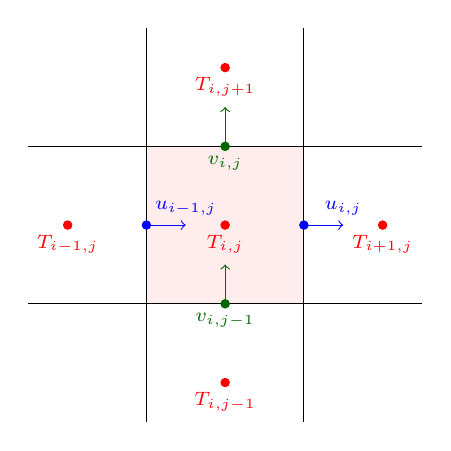
\begin{tikzpicture}[scale=1, style={font=\scriptsize}]
	\tikzset{dimen/.style={<->,>=latex,thin,every rectangle node/.style={fill=white,midway,font=\small}}}
	
	\filldraw[red!7] (0,0) -- (2,0) -- (2,2) -- (0, 2) -- cycle;
	\draw (-1.5, 0) -- (3.5, 0);
	\draw (-1.5, 2) -- (3.5, 2);
	\draw (0, -1.5) -- (0, 3.5);
	\draw (2, -1.5) -- (2, 3.5);
	
	\filldraw[red] (1, 1) circle (1.5pt);
	\filldraw[blue] (0, 1) circle (1.5pt);
	\filldraw[green!40!black] (1, 0) circle (1.5pt);
	\filldraw[blue] (2, 1) circle (1.5pt);
	\filldraw[green!40!black] (1, 2) circle (1.5pt);
	\filldraw[red] (-1, 1) circle (1.5pt);
	\filldraw[red] (3, 1) circle (1.5pt);
	\filldraw[red] (1, 3) circle (1.5pt);
	\filldraw[red] (1, -1) circle (1.5pt);
	
	\draw [->,blue] (0, 1) -- (0.5, 1);
	\draw [->,blue] (2, 1) -- (2.5, 1);
	\draw [->,green!40!black] (1, 0) -- (1,0.5);
	\draw [->,green!40!black] (1, 2) -- (1,2.5);
	
	\node[below, red] at (1, 1) {$T_{i, j}$};
	\node[below, red] at (3, 1) {$T_{i+1, j}$};
	\node[below, red] at (-1, 1) {$T_{i-1, j}$};
	\node[below, red] at (1, 3) {$T_{i, j+1}$};
	\node[below, red] at (1, -1) {$T_{i, j-1}$};
	
	\node[above,blue] at (0.5, 1) {$u_{i-1,j}$};
	\node[above,blue] at (2.5, 1) {$u_{i,j}$};
	\node[below,green!40!black] at (1, 0) {$v_{i,j-1}$};
	\node[below,green!40!black] at (1, 2) {$v_{i,j}$};
	\end{tikzpicture}
	\caption{An internal temperature control volume.}
	\label{fig:CV-T}
\end{figure}

The integration of the energy equation equations using the power-law scheme results in the equation (for $i = 1, \ldots, M_x^T - 1\,\,,\, j = 1, \ldots, M_y^T - 1$)
\begin{subequations}
	\label{eq:power}
	\begin{align}
	a^{T_{i,j}}_p T_{i,j} & = a^{\phi_{i,j}}_n T_{i, j+1} + a^{\phi_{i,j}}_e T_{i+1, j} + a^{T_{i,j}}_s T^*_{i, j-1} + a^{T_{i,j}}_w T_{i-1, j} \,,\\
	a^{T_{i,j}}_n & = D^{T_{i,j}}_n \max \left[0, (1 - 0.1 |F^{T_{i,j}}_n/D^{T_{i,j}}_n|)^5\right] + \max \left[ -F^{T_{i,j}}_n, 0 \right]\,, \\
	a^{T_{i,j}}_e & = D^{T_{i,j}}_e \max \left[0, (1 - 0.1 |F^{T_{i,j}}_e/D^{T_{i,j}}_e|)^5\right] + \max \left[ -F^{T_{i,j}}_e, 0 \right]\,, \\
	a^{T_{i,j}}_s & = D^{T_{i,j}}_s \max \left[0, (1 - 0.1 |F^{T_{i,j}}_s/D^{T_{i,j}}_s|)^5\right] + \max \left[ F^{T_{i,j}}_s, 0 \right]\,, \\
	a^{T_{i,j}}_w & = D^{T_{i,j}}_w \max \left[0, (1 - 0.1 |F^{T_{i,j}}_w/D^{T_{i,j}}_w|)^5\right] + \max \left[ F^{T_{i,j}}_w, 0 \right]\,, \\
	a^{T_{i,j}}_p & = a^{T_{i,j}}_n + a^{T_{i,j}}_e + a^{T_{i,j}}_s + a^{T_{i,j}}_w\,.
	\end{align}
\end{subequations}
The flow rates are defined as
\begin{subequations}
	\begin{align}
		F^{T_{i,j}}_n & = \rho C_p \Delta x v_{i,j}\,,\\
		F^{T_{i,j}}_e & = \rho C_p \Delta x u_{i,j}\,,\\
		F^{T_{i,j}}_s & = \rho C_p \Delta x v_{i,j - 1}\,,\\
		F^{T_{i,j}}_w & = \rho C_p \Delta x u_{i - 1,j}\,,
	\end{align}
\end{subequations}
and the ``diffusion'' coefficients are defined as
\begin{subequations}
	\begin{align}
		D^{T_{i,j}}_n & = k \begin{cases} \frac{2\Delta x}{\Delta y}\,, & j = M_y^T - 1 \\ \frac{\Delta x}{\Delta y} & \text{otherwise}\end{cases}\,,\\
		D^{T_{i,j}}_e & = k \begin{cases} \frac{2\Delta y}{\Delta x}\,, & i = M_x^T - 1 \\ \frac{\Delta y}{\Delta x} & \text{otherwise}\end{cases}\,,\\
		D^{T_{i,j}}_s & = k \begin{cases} \frac{2\Delta x}{\Delta y}\,, & j = 1 \\ \frac{\Delta x}{\Delta y} & \text{otherwise}\end{cases}\,,\\
		D^{T_{i,j}}_w & = k \begin{cases} \frac{2\Delta y}{\Delta x}\,, & i = 1 \\ \frac{\Delta y}{\Delta x} & \text{otherwise}\end{cases}\,.
	\end{align}
\end{subequations}

\section{Results}

\subsection{Problem 3: 10 $\times$ 5 grid}

The results requested for problem 3 follow in Tables \ref{table:coarse-u}, \ref{table:coarse-p-p0}, and \ref{table:coarse-T}.

\def\arraystretch{1.3}
\begin{table}[H]
	\scriptsize
	\centering
	\caption{The $u$-velocity solution with the 10 $\times$ 5 grid. A row corresponds to a $x$-position and a column corresponds to an $y$-position.}
	\vspace{0.2cm}
	\sisetup{output-exponent-marker = \text{E}, table-format=2.5e1,group-digits=false,retain-zero-exponent=true}
	\begin{tabular}{c|S|S|S|S|S|S|S}
		& {1} & {2} & {3} & {4} & {5} & {6} & {7} \\
		\hline
        1 & 5.06931e-03 & 5.06931e-03 & 5.06931e-03 & 5.06931e-03 & 5.06931e-03 & 5.06931e-03 & 5.06931e-03 \\
        2 & 0.00000e+00 & 3.02156e-03 & 6.10805e-03 & 7.08733e-03 & 6.10805e-03 & 3.02156e-03 & 0.00000e+00 \\
        3 & 0.00000e+00 & 2.84164e-03 & 6.18930e-03 & 7.28469e-03 & 6.18930e-03 & 2.84164e-03 & 0.00000e+00 \\
        4 & 0.00000e+00 & 2.81967e-03 & 6.19551e-03 & 7.31618e-03 & 6.19551e-03 & 2.81967e-03 & 0.00000e+00 \\
        5 & 0.00000e+00 & 2.81677e-03 & 6.19585e-03 & 7.32132e-03 & 6.19585e-03 & 2.81677e-03 & 0.00000e+00 \\
        6 & 0.00000e+00 & 2.81636e-03 & 6.19583e-03 & 7.32217e-03 & 6.19583e-03 & 2.81636e-03 & 0.00000e+00 \\
        7 & 0.00000e+00 & 2.81630e-03 & 6.19583e-03 & 7.32231e-03 & 6.19583e-03 & 2.81630e-03 & 0.00000e+00 \\
        8 & 0.00000e+00 & 2.81629e-03 & 6.19582e-03 & 7.32233e-03 & 6.19582e-03 & 2.81629e-03 & 0.00000e+00 \\
        9 & 0.00000e+00 & 2.81628e-03 & 6.19582e-03 & 7.32234e-03 & 6.19582e-03 & 2.81628e-03 & 0.00000e+00 \\
        10 & 0.00000e+00 & 2.81628e-03 & 6.19582e-03 & 7.32234e-03 & 6.19582e-03 & 2.81628e-03 & 0.00000e+00 \\
        11 & 0.00000e+00 & 2.81628e-03 & 6.19582e-03 & 7.32234e-03 & 6.19582e-03 & 2.81628e-03 & 0.00000e+00 \\
	\end{tabular}
	\label{table:coarse-u}
\end{table}

\def\arraystretch{1.3}
\begin{table}[H]
	\scriptsize
	\centering
	\caption{The $(P - P_0)$ solution with the 10 $\times$ 5 grid. A row corresponds to a $x$-position and a column corresponds to an $y$-position.}
	\vspace{0.2cm}
	\sisetup{output-exponent-marker = \text{E}, table-format=2.5e1,group-digits=false,retain-zero-exponent=true}
	\begin{tabular}{c|S|S|S|S|S|S|S}
		& {1} & {2} & {3} & {4} & {5} & {6} & {7} \\
		\hline
        1 & 2.88374e-01 & 2.88374e-01 & 2.88353e-01 & 2.88346e-01 & 2.88353e-01 & 2.88374e-01 & 2.88374e-01 \\
        2 & 2.88374e-01 & 2.88374e-01 & 2.88353e-01 & 2.88346e-01 & 2.88353e-01 & 2.88374e-01 & 2.88374e-01 \\
        3 & 2.40648e-01 & 2.40648e-01 & 2.40651e-01 & 2.40653e-01 & 2.40651e-01 & 2.40648e-01 & 2.40648e-01 \\
        4 & 2.11749e-01 & 2.11749e-01 & 2.11750e-01 & 2.11750e-01 & 2.11750e-01 & 2.11749e-01 & 2.11749e-01 \\
        5 & 1.83440e-01 & 1.83440e-01 & 1.83440e-01 & 1.83440e-01 & 1.83440e-01 & 1.83440e-01 & 1.83440e-01 \\
        6 & 1.55208e-01 & 1.55208e-01 & 1.55208e-01 & 1.55208e-01 & 1.55208e-01 & 1.55208e-01 & 1.55208e-01 \\
        7 & 1.26987e-01 & 1.26987e-01 & 1.26987e-01 & 1.26987e-01 & 1.26987e-01 & 1.26987e-01 & 1.26987e-01 \\
        8 & 9.87671e-02 & 9.87671e-02 & 9.87671e-02 & 9.87671e-02 & 9.87671e-02 & 9.87671e-02 & 9.87671e-02 \\
        9 & 7.05479e-02 & 7.05479e-02 & 7.05479e-02 & 7.05479e-02 & 7.05479e-02 & 7.05479e-02 & 7.05479e-02 \\
        10 & 4.23287e-02 & 4.23287e-02 & 4.23287e-02 & 4.23287e-02 & 4.23287e-02 & 4.23287e-02 & 4.23287e-02 \\
        11 & 0.00000e+00 & 0.00000e+00 & 0.00000e+00 & 0.00000e+00 & 0.00000e+00 & 0.00000e+00 & 0.00000e+00 \\
        12 & 0.00000e+00 & 0.00000e+00 & 0.00000e+00 & 0.00000e+00 & 0.00000e+00 & 0.00000e+00 & 0.00000e+00 \\
	\end{tabular}
	\label{table:coarse-p-p0}
\end{table}

\def\arraystretch{1.3}
\begin{table}[H]
	\scriptsize
	\centering
	\caption{The $T$ solution with the 10 $\times$ 5 grid. A row corresponds to a $x$-position and a column corresponds to an $y$-position.}
	\vspace{0.2cm}
	\sisetup{table-format=2.5,group-digits=false}
	\begin{tabular}{c|S|S|S|S|S|S|S}
		& {1} & {2} & {3} & {4} & {5} & {6} & {7} \\
		\hline
        1 & 26.64204 & 25.00000 & 25.00000 & 25.00000 & 25.00000 & 25.00000 & 26.64204 \\
        2 & 27.69621 & 26.05418 & 25.36548 & 25.17769 & 25.36548 & 26.05418 & 27.69621 \\
        3 & 28.84253 & 27.20050 & 25.72681 & 25.36877 & 25.72681 & 27.20050 & 28.84253 \\
        4 & 29.72586 & 28.08382 & 26.15140 & 25.63232 & 26.15140 & 28.08382 & 29.72586 \\
        5 & 30.44158 & 28.79955 & 26.60972 & 25.95974 & 26.60972 & 28.79955 & 30.44158 \\
        6 & 31.06105 & 29.41902 & 27.08232 & 26.33547 & 27.08232 & 29.41902 & 31.06105 \\
        7 & 31.62445 & 29.98241 & 27.56009 & 26.74529 & 27.56009 & 29.98241 & 31.62445 \\
        8 & 32.15448 & 30.51244 & 28.03926 & 27.17831 & 28.03926 & 30.51244 & 32.15448 \\
        9 & 32.66429 & 31.02226 & 28.51841 & 27.62677 & 28.51841 & 31.02226 & 32.66429 \\
        10 & 33.16165 & 31.51962 & 28.99712 & 28.08535 & 28.99712 & 31.51962 & 33.16165 \\
        11 & 33.65119 & 32.00915 & 29.47532 & 28.55050 & 29.47532 & 32.00915 & 33.65119 \\
        12 & 33.89596 & 32.25392 & 29.71442 & 28.78307 & 29.71442 & 32.25392 & 33.89596 \\
	\end{tabular}
	\label{table:coarse-T}
\end{table}

\subsection{Problem 4: 180 $\times$ 54 grid}

The requirements for problem (b) part i and ii were combined into Figure \ref{fig:p2} as seen below. With increasing grid refinement, both centerline velocity profiles approached towards the reference solution obtained from Roy et. al. In addition, a once-more-refined run is compared with 256x256 CVs with good agreement.

\begin{figure}[H]
	\centering
	\includegraphics[width=0.75\linewidth]{../results/u_centerline}
	\caption{$u/u_\mathrm{in}$ plotted along the centerline of the channel for the 180 $\times$ 54 grid.}
	\label{fig:u-centerline}
\end{figure}

\begin{figure}[H]
	\centering
	\includegraphics[width=0.75\linewidth]{../results/u_0p8}
	\caption{$u$ plotted at $x = 0.8$ m for the 180 $\times$ 54 grid.}
	\label{fig:u-0p8}
\end{figure}

\begin{figure}[H]
	\centering
	\includegraphics[width=0.75\linewidth]{../results/v_0p8}
	\caption{$v$ plotted at $x = 0.8$ m for the 180 $\times$ 54 grid.}
	\label{fig:v-0p8}
\end{figure}

\begin{figure}[H]
	\centering
	\includegraphics[width=0.75\linewidth]{../results/T_0p8}
	\caption{$T$ plotted at $x = 0.8$ m for the 180 $\times$ 54 grid.}
	\label{fig:T-0p8}
\end{figure}

\begin{figure}[H]
	\centering
	\includegraphics[width=0.75\linewidth]{../results/Nu}
	\caption{The Nusselt number plotted as a function of stream-wise distance for the 180 $\times$ 54 grid.}
	\label{fig:Nu}
\end{figure}

\section*{Code listing}

For the implementation, we have the following files:
\begin{itemize}
	\item \texttt{Makefile} -- Allows for compiling the c++ project with \texttt{make}.
	\item \texttt{hwk5.cpp} -- Contains the \texttt{main()} function that is required by C that runs the cases requested in this problem set.
	\item \texttt{Problem.h} -- Contains the header for the \texttt{Problem} class which is the main driver for a \texttt{Flow2D::Problem}.
	\item \texttt{Variable.h} -- Contains the \texttt{Flow2D::Variable} class, which is a storage container for a single variable (i.e., $u$).
	\item \texttt{Problem.cpp} -- Contains the \texttt{run()} functions that executes a \texttt{Problem}.
	\item \texttt{Problem\_coefficients.cpp} -- Contains the functions for solving coefficients in a \texttt{Problem}.
	\item \texttt{Problem\_corrections.cpp} -- Contains the functions for correcting solutions in a \texttt{Problem}.
	\item \texttt{Problem\_residuals.cpp} -- Contains the functions for computing residuals in a \texttt{Problem}.
	\item \texttt{Problem\_solvers.cpp} -- Contains the functions for sweeping and solving in a \texttt{Problem}.
	\item \texttt{Matrix.h} -- Contains the \texttt{Matrix} class which provides storage for a matrix with various standard matrix operations.
	\item \texttt{TriDiagonal.h} -- Contains the \texttt{TriDiagonal} class which provides storage for a tri-diagonal matrix including the TDMA solver found in the member function \texttt{solveTDMA()}.
	\item \texttt{Vector.h} -- Contains the \texttt{Vector} class for one-dimensional vector storage.
	\item \texttt{postprocess.py} - Produces the plots and tables in this report.
\end{itemize}

\subsection*{Makefile}
\inputminted[fontsize=\scriptsize]{Makefile}{../Makefile}

\subsection*{hwk5.cpp}
\inputminted[fontsize=\scriptsize]{c++}{../hwk5.cpp}

\newpage
\subsection*{Problem.h}
\inputminted[fontsize=\scriptsize]{c++}{../Problem.h}

\newpage
\subsection*{Variable.h}
\inputminted[fontsize=\scriptsize]{c++}{../Variable.h}

\newpage
\subsection*{Problem.cpp}
\inputminted[fontsize=\scriptsize]{c++}{../Problem.cpp}

\newpage
\subsection*{Problem\_coefficients.cpp}
\inputminted[fontsize=\scriptsize]{c++}{../Problem_coefficients.cpp}

\newpage
\subsection*{Problem\_corrections.cpp}
\inputminted[fontsize=\scriptsize]{c++}{../Problem_corrections.cpp}

\newpage
\subsection*{Problem\_residuals.cpp}
\inputminted[fontsize=\scriptsize]{c++}{../Problem_residuals.cpp}

\newpage
\subsection*{Problem\_solvers.cpp}
\inputminted[fontsize=\scriptsize]{c++}{../Problem_solvers.cpp}

\newpage
\subsection*{Matrix.h}
\inputminted[fontsize=\scriptsize]{c++}{../Matrix.h}

\newpage
\subsection*{TriDiagonal.h}
\inputminted[fontsize=\scriptsize]{c++}{../TriDiagonal.h}

\newpage
\subsection*{Vector.h}
\inputminted[fontsize=\scriptsize]{c++}{../Vector.h}

\newpage
\subsection*{postprocess.py}
\inputminted[fontsize=\scriptsize]{python}{../postprocess.py}

\end{document}
